\section{Construction of Experiment and used Devices}
Central part of our experiment is a cell with the rubidium gas in it, which we want to investigate. In its normal compound, natural rubidium consists of $72\%$ $^{85}Rb$ and $28\%$ $ ^{87}Rb$, so we have both isotopes in the cell.

We also need a lamp, from which we radiate the light to the rubidium cell. In the direct opposite of the lamp, we have a detector to measure the incoming and therefore not absorbed radiation. The signal of the detector is shown by an oscilloscope, where we can do our measurements of the signal. Of course, we have to use polarized light of a special wavelength for optical pumping, while the light of the lamp is unpolarized. So we have three filters in the beam between the lamp and the Rb-cell. This and the following setup can be seen in figure \ref{setup} The first filter selects one special wavelength wich can pass the filter, other wavelengths are deflected. The next filter polarizes the incoming light linearly, so it can be polarized circular more easily. That can be reached by the third filter, which is a so-called $\frac{\lambda}{4}$-plate. This is mainly a cristal with a special grid distance, which delays one part of the radiation wave and has no effect to the other part. After that filter, we have a right-handed circular polarized light of a certain wavelength, as we need to realize optical pumping. Also, our beam is focused twice by lenses, once for aiming the radiation in the Rb-cell and afterwards to be focused in the detector. 

In our experiment, we need different magnetic fields, so we have three pairs of helmholtz coils aroung the rubidium cell. One of it generates a field in vertical direction, while the other two pairs generate horizontal fields. The coil pairs are driven  either by a programmable DC power supply or a function generator for AC currents. Depending on the connected device, we can generate constant or oscillating magnetic fields. 

Additionally, we heat our Rb-cell with a little heating system, so the Rb-atoms are completely in gas state. 

\begin{figure}[htbp] 
     \usetikzlibrary{shapes,arrows}
\tikzstyle{block1} = [draw, fill=blue!20, rectangle, 
    minimum height=3em, minimum width=4em, text width=1cm]
\tikzstyle{block2}=[draw, fill=blue!0,rectangle, minimum height=3em, minimum width=4em, text width=1cm]
\tikzstyle{lense} = [draw, fill=blue!00, ellipse, 
    minimum height=6em, minimum width=2em]
\tikzstyle{filter}=[draw, fill=black!40,rectangle, minimum height=4.5em, minimum width=0.3em]
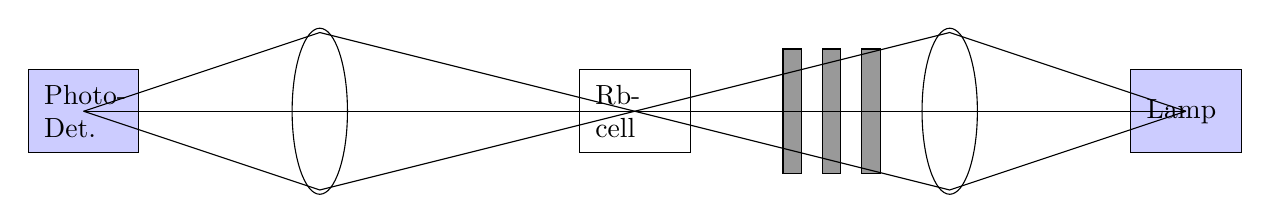
\begin{tikzpicture}
\coordinate (O) at (0,0);
\coordinate (L0) at (-7,0);
\coordinate (L1) at (-4,0);
\coordinate (R0) at (2,0);
\coordinate (R1) at (2.5,0);
\coordinate (R2) at (3,0);
\coordinate (R3) at (4,0);
\coordinate (R4) at (7,0);

\node[block1, name=det] at (L0) {Photo-Det.};
\node[lense, name=lense1] at (L1){};
\node[block2, name=cell] at (O){Rb-cell};
\node[filter, name=f1] at (R0){};
\node[filter, name=f2] at (R1){};
\node[filter, name=f3] at (R2){};
\node[lense, name=lense2] at (R3){};
\node[block1, name=lamp] at (R4){Lamp};
\draw (L0) -- (R4);
\draw (L0) -- (-4,1) -- (4,-1) -- (R4);
\draw (L0) -- (-4,-1) -- (4,1) -- (R4);
\end{tikzpicture}
  \caption{Schematical setup of the experiment}
  \label{setup}
\end{figure}
